\documentclass[12pt,a4paper]{article}
\usepackage[margin=1.5cm]{geometry}
\usepackage[T1]{fontenc}
\usepackage[utf8]{inputenc}
\usepackage{lmodern}
\usepackage{booktabs}
\usepackage{tabularx}
\usepackage{array}
\usepackage{enumitem}
\usepackage{xcolor}
\usepackage{hyperref}
\usepackage{microtype}
\usepackage{tikz}
\usetikzlibrary{shapes.geometric, arrows.meta, positioning, calc, fit, backgrounds, decorations.pathreplacing}

\definecolor{brand}{HTML}{176B52}
\definecolor{brandlight}{HTML}{E8F4F0}
\definecolor{branddark}{HTML}{0E4D3B}
\definecolor{muted}{HTML}{5F716B}
\definecolor{accent}{HTML}{D97706}
\definecolor{warningbg}{HTML}{FFFBEB}
\definecolor{alertred}{HTML}{B91C1C}

\hypersetup{colorlinks=true,linkcolor=brand,urlcolor=brand,citecolor=brand}
\setlength{\parindent}{0pt}
\setlength{\parskip}{0.55em}
\newcommand{\status}[1]{\textbf{\color{brand}[#1]}}
\newcommand{\code}[1]{\texttt{#1}}

% TikZ Diagram Styles
\tikzset{
  umlclass/.style = {rectangle, draw=branddark, fill=white, minimum width=3.4cm, text width=3.2cm, inner sep=0.2cm, font=\scriptsize},
  umlheader/.style = {rectangle, draw=branddark, fill=brandlight, minimum width=3.4cm, text width=3.2cm, inner sep=0.15cm, text centered, font=\scriptsize\bfseries},
  layerbox/.style = {rectangle, rounded corners=3pt, draw=brand, fill=brandlight, minimum width=15cm, minimum height=1.3cm, text width=14.6cm, inner sep=0.25cm, font=\footnotesize},
  flowbox/.style = {rectangle, rounded corners=3pt, draw=brand, fill=brandlight, minimum width=2.6cm, minimum height=0.9cm, text centered, text width=2.5cm, font=\footnotesize\bfseries},
  flowproc/.style = {rectangle, rounded corners=2pt, draw=brand!80, fill=white, minimum width=2.5cm, minimum height=0.8cm, text centered, text width=2.4cm, font=\scriptsize},
  flowdec/.style = {diamond, aspect=1.8, draw=brand, fill=warningbg, minimum width=2.2cm, minimum height=0.8cm, text centered, text width=1.9cm, font=\scriptsize\bfseries},
  flowarrow/.style = {thick, -{Stealth[length=2.2mm]}, draw=brand},
  dashedarrow/.style = {thick, dashed, -{Stealth[length=2.2mm]}, draw=muted}
}

\title{\textbf{Footprint Lens: Architectural Design, Project Planning and Evaluation Protocol}\\[0.4em]
  \large COMP2300 Deliverable 3 Technical Report\\
  \normalsize High-Fidelity Evaluation Strategy, Java/JavaFX Clean Architecture, Agile Scrum Plan, and Risk Management}
\author{Arnav Mishra \and Keshav Singhal \and Hiranya Makkar\\[0.4em]
  \small Department of Electronics and Computer Science, University of Southampton}
\date{November 2026}

\begin{document}
\maketitle

\begin{abstract}
\noindent Deliverable 3 formalizes the engineering blueprint, agile management framework, and summative evaluation strategy for \textbf{Footprint Lens}, an interactive carbon awareness tool developed for COMP2300 Topic 1. Grounded in the conceptual design of Deliverable 2, this report addresses all four criteria of the D3 assessment rubric at the Distinction (80+) benchmark. First, we specify a user-centred, lab-based evaluation plan involving moderated think-aloud usability testing with peers recruited from an independent COMP2300 group, adhering strictly to UK GDPR Special Category data restrictions. Second, we present an exhaustive technical architecture using Java 21 LTS and JavaFX 21, structured into Presentation, Application, Domain, and Persistence layers. We document the system using formal vector UML Package, Class, and Sequence diagrams, justifying key decisions regarding headless testability, immutable domain records, and non-speculative deterministic rule engines. Third, we articulate an agile Scrum implementation plan spanning four structured sprints, detailing the Sprint 1 backlog, story points, acceptance criteria, and a formal burndown chart. Finally, we document the development setup, GitLab workflow, and an eight-factor risk management register with concrete mitigation strategies.
\end{abstract}

\hrule
\vspace{0.8em}

\section{Introduction and System Scope}
Deliverable 2 established the conceptual foundations of \textbf{Footprint Lens (Concept A: Contextual Choice Coach)}, demonstrating through low-fidelity prototypes that urban Indian householders require transparent assumption provenance, constraint-protected routines, and communal-versus-individual boundary protection. Deliverable 3 translates this concept into an implementable, maintainable, and verifiable software engineering system. 

The primary technical objective of D3 is to establish an architectural foundation that supports automated testing of business logic independent of graphical UI harnesses, delivers value in incremental sprint cycles, and prepares a rigorous, ethical evaluation protocol for the final high-fidelity software release in D7.

\section{Summative Evaluation Plan for High-Fidelity Prototype}

\subsection{Evaluation Methodology and Setting}
To evaluate the final high-fidelity system at the culmination of the project (D7), the team has formulated an empirical, user-centred evaluation plan. In strict compliance with the COMP2300 specification, the evaluation employs a \textbf{moderated, task-based usability testing protocol combined with a think-aloud procedure} \cite{lasarov2024}. 

Heuristic evaluation is recognized as an expert review technique and is explicitly excluded as a standalone method; it may only serve as an internal preliminary check. The evaluation will take place in a \textbf{controlled lab environment} (a quiet, booked study room on campus), ensuring consistent ambient lighting, acoustic isolation, and zero external distractions. Remote testing and ``in-the-wild'' unmoderated trials are excluded to maintain experimental control.

\subsection{Participant Recruitment and Ethical Safeguards (UK GDPR)}
In accordance with course regulations:
\begin{itemize}[leftmargin=*]
  \item \textbf{Recruitment Target:} $N = 6$ participants recruited directly by the team from another COMP2300 project group. This peer cohort provides participants with appropriate technical literacy who are familiar with coursework contexts but completely naive to our codebase and interface.
  \item \textbf{Data Protection and UK GDPR Compliance:} Under the UK General Data Protection Regulation (UK GDPR, Section 9) \cite{ico2024}, the study strictly prohibits collecting or eliciting any \emph{Special Category Data} (such as health conditions, religious beliefs, political affiliations, sexual orientation, or biometrics). Furthermore, to eliminate privacy risks in shared housing, participants will \textbf{never} be asked to input their real utility bills, bank statements, income, or live home addresses.
  \item \textbf{Standardized Synthetic Scenarios:} All experimental tasks utilize pre-constructed synthetic activity cards (e.g., standardized 150~kWh electricity bills or 15~km night commutes) to ensure full reproducibility and zero personal data leakage.
  \item \textbf{Consent and Anonymization:} Participants will receive an Information Sheet and sign an Informed Consent Script prior to testing. Observational logs will use anonymized identifiers (\code{P01}--\code{P06}).
\end{itemize}

\subsection{Standardized Task Protocol}
Participants will execute five core task scenarios designed to stress-test the D1/D2 epics (E1--E5, E7):

\begin{table}[ht]
\centering
\small
\caption{Structured Evaluation Task Scenarios and Success Criteria}
\begin{tabularx}{\textwidth}{@{}p{1.2cm}p{4.0cm}p{5.5cm}X@{}}
\toprule
\textbf{Task} & \textbf{Scenario Prompt} & \textbf{Expected Participant Interaction} & \textbf{Observable Success Gate}\\
\midrule
\textbf{T1 (E1)} & ``Log a monthly home electricity use of 150~kWh for your personal room.'' & Select Electricity $\rightarrow$ Scope: Personal $\rightarrow$ Input 150 $\rightarrow$ Submit $\rightarrow$ View Result. & Correctly identifies numeric estimate and INR variable cost comparison.\\
\textbf{T2 (E2)} & ``Inspect how the app calculated this number and what data year it uses.'' & From P2 Result, click ``Inspect assumptions'' $\rightarrow$ Review P3 Table. & Accurately states conversion factor (0.716), source, and 2026 reference year.\\
\textbf{T3 (E3)} & ``Log a 15~km auto-rickshaw commute taken at night due to personal safety.'' & Select Travel $\rightarrow$ Enter 15~km $\rightarrow$ Check ``Protected/necessary'' $\rightarrow$ View P4 Action. & Understands why action decisions are disabled; confirms absence of preachy blame.\\
\textbf{T4 (E4)} & ``Log 3~kg of weekly delivery packaging from online food orders.'' & Select Packaging $\rightarrow$ Enter 3~kg $\rightarrow$ View Result and Unknown Explanation (P5). & Recognizes that descriptive log is preserved without fabricating false carbon offsets.\\
\textbf{T5 (E7)} & ``Inspect a 500~kWh communal flat electricity bill on the Shared Total view.'' & From Result, navigate to P6 (Shared Total) $\rightarrow$ Inspect communal boundary. & Accurately explains back that household total cannot be attributed to one person.\\
\bottomrule
\end{tabularx}
\end{table}

\subsection{Quantitative Metrics and Qualitative Analysis}
\begin{itemize}[leftmargin=*]
  \item \textbf{Task Effectiveness:} Task Completion Rate (binary success without moderator intervention); Critical Error Rate (submitting invalid data without self-recovery).
  \item \textbf{Efficiency:} Time on Task (target: $\le 60$ seconds for T1; $\le 90$ seconds for T2--T5).
  \item \textbf{Subjective Usability:} Post-task Single Ease Question (SEQ, 1--7 scale); post-test System Usability Scale (SUS) questionnaire with a benchmark target of $\ge 75/100$ (Grade A- / Distinction).
  \item \textbf{Cognitive Comprehension Probes:} Semi-structured explain-back questions evaluating whether participants understood that illustrative numbers are not verified emissions.
  \item \textbf{Data Analysis Plan:} Quantitative measures will be summarized using descriptive statistics (medians, interquartile ranges, explicit completion ratios). Qualitative think-aloud utterances and observer notes will be transcribed and evaluated using thematic analysis to identify usability friction points.
\end{itemize}

\section{Technical Architecture and Design Justification}

\subsection{Architectural Paradigm: Clean Layered Architecture}
The Footprint Lens application is engineered following the \textbf{Clean Layered Architecture} pattern (Figure~\ref{fig:layered_arch}). The architecture establishes strict unidirectional dependency constraints: presentation depends on application services, which depend on domain models, while domain models remain completely agnostic of UI frameworks and persistence mechanisms.

\begin{figure}[ht]
\centering
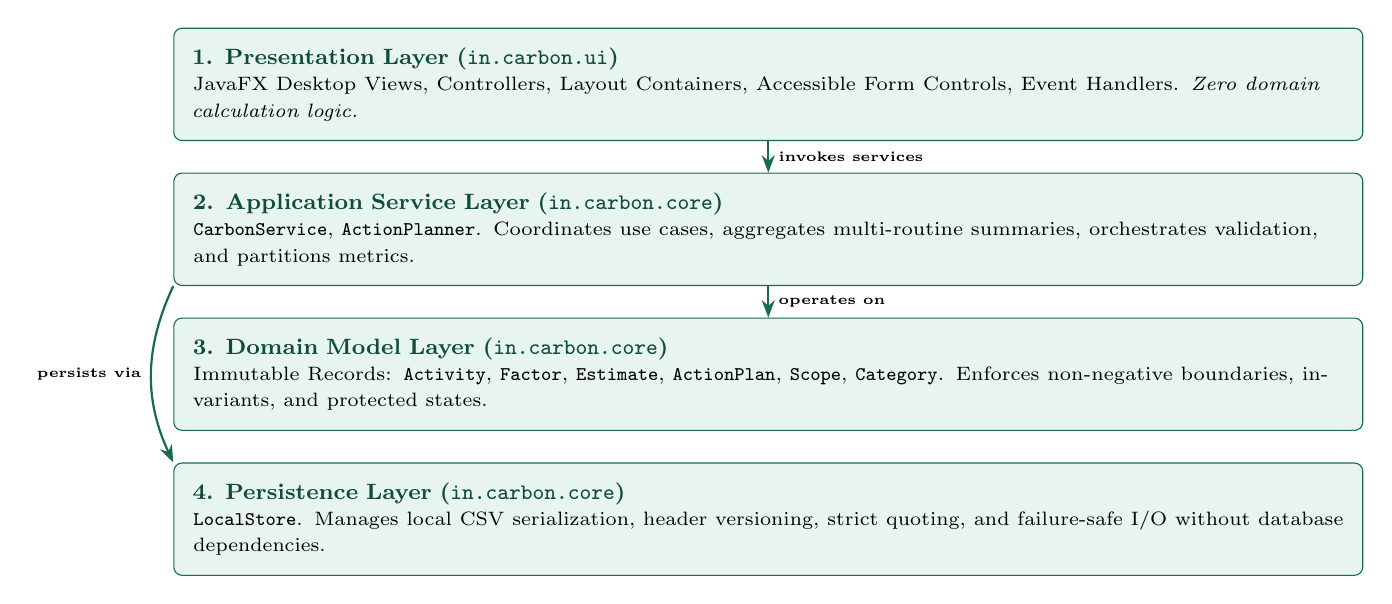
\begin{tikzpicture}[node distance=0.5cm]
  \node[layerbox] (ui) {
    \textbf{\color{branddark}1. Presentation Layer (\code{in.carbon.ui})}\\
    \scriptsize JavaFX Desktop Views, Controllers, Layout Containers, Accessible Form Controls, Event Handlers. \emph{Zero domain calculation logic.}
  };
  \node[layerbox, below=0.4cm of ui] (app) {
    \textbf{\color{branddark}2. Application Service Layer (\code{in.carbon.core})}\\
    \scriptsize \code{CarbonService}, \code{ActionPlanner}. Coordinates use cases, aggregates multi-routine summaries, orchestrates validation, and partitions metrics.
  };
  \node[layerbox, below=0.4cm of app] (domain) {
    \textbf{\color{branddark}3. Domain Model Layer (\code{in.carbon.core})}\\
    \scriptsize Immutable Records: \code{Activity}, \code{Factor}, \code{Estimate}, \code{ActionPlan}, \code{Scope}, \code{Category}. Enforces non-negative boundaries, invariants, and protected states.
  };
  \node[layerbox, below=0.4cm of domain] (persist) {
    \textbf{\color{branddark}4. Persistence Layer (\code{in.carbon.core})}\\
    \scriptsize \code{LocalStore}. Manages local CSV serialization, header versioning, strict quoting, and failure-safe I/O without database dependencies.
  };

  \draw[flowarrow] (ui) -- node[right, font=\tiny\bfseries] {invokes services} (app);
  \draw[flowarrow] (app) -- node[right, font=\tiny\bfseries] {operates on} (domain);
  \draw[flowarrow] (app.south west) to[bend right=25] node[left, font=\tiny\bfseries] {persists via} (persist.north west);
\end{tikzpicture}
\caption{Four-Tier Layered Architecture of Footprint Lens}
\label{fig:layered_arch}
\end{figure}

\subsection{Key Architectural Decisions and Justifications}
\begin{enumerate}[label=\textbf{AD\arabic*.},leftmargin=*]
  \item \textbf{Decoupled Domain from JavaFX (Headless Testability):} The domain layer contains zero references to \code{javafx.*} classes. This allows the complete business logic, mathematical formulas, and boundary validations to be executed in continuous integration pipelines using JUnit 5 without requiring a virtual display server (Xvfb) or graphical runner.
  \item \textbf{Immutable Domain Records and Arbitrary-Precision Math:} Domain entities (\code{Activity}, \code{Factor}, \code{Estimate}) are implemented as Java 21 \code{record}s. All numerical calculations utilize \code{java.math.BigDecimal} rather than floating-point primitives (\code{double}), completely eliminating binary IEEE-754 floating-point rounding errors in carbon accounting.
  \item \textbf{Metric-Partitioned Aggregations:} In \code{CarbonService.totalsByMetric()}, totals are strictly partitioned by metric type (\code{CO2} vs \code{CO2E}). The system enforces an architectural invariant prohibiting the silent addition of distinct greenhouse gas metrics.
  \item \textbf{Deterministic Rule Engine vs. Speculative Machine Learning:} In strict alignment with course guidelines prohibiting speculative machine learning, \code{ActionPlanner} utilizes a transparent, deterministic rule-matching engine. Every recommendation is traceable to explicit preconditions, ensuring complete auditability.
  \item \textbf{Versioned Local File Persistence:} To eliminate external server, cloud database, or container setup barriers, persistence is handled by \code{LocalStore} using versioned, RFC-4180-compliant CSV files with strict header verification (\code{FOOTPRINT-LENS,1}).
\end{enumerate}

\subsection{UML Class Diagram}
Figure~\ref{fig:uml_class} documents the complete class model, attributes, operations, and relationships across the core domain and presentation layers.

\begin{figure}[ht]
\centering
\begin{tikzpicture}[node distance=0.8cm and 0.6cm]
  % CarbonService
  \node[umlheader] (cshead) {CarbonService};
  \node[umlclass, below=0cm of cshead] (csbody) {
    + estimate(Activity): Estimate\\
    + totalsByMetric(List): Map\\
    + waterBuckets(BigDecimal): BigDecimal
  };
  \node[fit={(cshead)(csbody)}, inner sep=0pt] (cs) {};

  % ActionPlanner
  \node[umlheader, right=1.0cm of cshead] (aphead) {ActionPlanner};
  \node[umlclass, below=0cm of aphead] (apbody) {
    + suggestion(Activity): Optional\\
    - isEligible(Activity, Rule): boolean
  };
  \node[fit={(aphead)(apbody)}, inner sep=0pt] (ap) {};

  % Activity Record
  \node[umlheader, below=1.2cm of csbody] (acthead) {Activity \guillemotleft record\guillemotright};
  \node[umlclass, below=0cm of acthead] (actbody) {
    - id: String\\
    - category: Category\\
    - quantity: BigDecimal\\
    - scope: Scope\\
    - protectedChoice: boolean\\
    - factor: Factor\\
    + estimate(): Estimate\\
    + displayName(): String
  };
  \node[fit={(acthead)(actbody)}, inner sep=0pt] (act) {};

  % Factor Record
  \node[umlheader, right=1.0cm of acthead] (facthead) {Factor \guillemotleft record\guillemotright};
  \node[umlclass, below=0cm of facthead] (factbody) {
    - value: BigDecimal\\
    - denominatorUnit: String\\
    - metric: String\\
    - source: String\\
    - year: String\\
    - status: FactorStatus\\
    + summary(): String
  };
  \node[fit={(facthead)(factbody)}, inner sep=0pt] (fact) {};

  % Estimate Record
  \node[umlheader, below=1.2cm of actbody] (esthead) {Estimate \guillemotleft record\guillemotright};
  \node[umlclass, below=0cm of esthead] (estbody) {
    - available: boolean\\
    - value: BigDecimal\\
    - metric: String\\
    - explanation: String\\
    + numeric(...): Estimate\\
    + unavailable(...): Estimate
  };
  \node[fit={(esthead)(estbody)}, inner sep=0pt] (est) {};

  % LocalStore
  \node[umlheader, right=1.0cm of esthead] (storehead) {LocalStore};
  \node[umlclass, below=0cm of storehead] (storebody) {
    - path: Path\\
    + save(List$<$Activity$>$): void\\
    + load(): List$<$Activity$>$\\
    - formatCsv(Activity): String
  };
  \node[fit={(storehead)(storebody)}, inner sep=0pt] (store) {};

  % Relationships
  \draw[flowarrow] (cs) -- (act);
  \draw[flowarrow] (ap) -- (act);
  \draw[flowarrow] (act) -- (fact);
  \draw[flowarrow] (act) -- (est);
  \draw[flowarrow] (store) -- (act);
\end{tikzpicture}
\caption{UML Class Diagram of Footprint Lens Domain Model and Services}
\label{fig:uml_class}
\end{figure}

\subsection{UML Sequence Diagram}
Figure~\ref{fig:uml_seq} illustrates the sequence of interactions when a user enters an activity in the JavaFX UI, triggering validation, calculation, constraint protection, and local persistence.

\begin{figure}[ht]
\centering
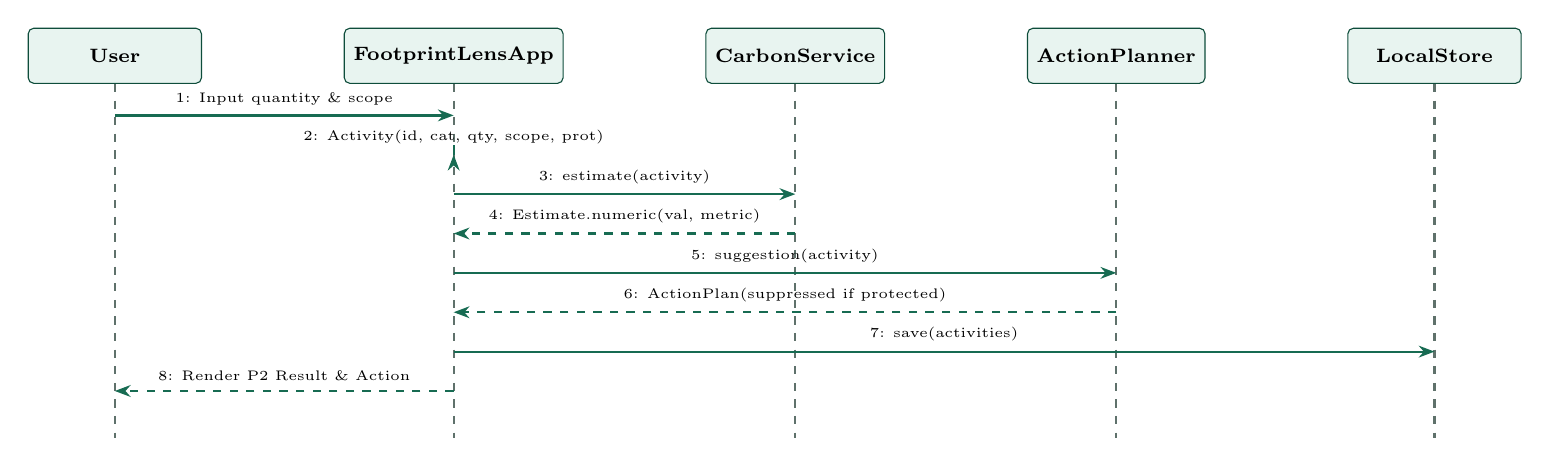
\begin{tikzpicture}[
  lifeline/.style = {dashed, draw=muted, thick},
  entity/.style = {rectangle, rounded corners=2pt, draw=branddark, fill=brandlight, minimum width=2.2cm, minimum height=0.7cm, text centered, font=\scriptsize\bfseries},
  call/.style = {thick, -{Stealth[length=2mm]}, draw=brand},
  ret/.style = {thick, dashed, -{Stealth[length=2mm]}, draw=brand}
]
  % Lifelines
  \node[entity] (u) {User};
  \node[entity, right=1.8cm of u] (ui) {FootprintLensApp};
  \node[entity, right=1.8cm of ui] (cs) {CarbonService};
  \node[entity, right=1.8cm of cs] (ap) {ActionPlanner};
  \node[entity, right=1.8cm of ap] (ls) {LocalStore};

  \coordinate (u_b) at ($(u.south) + (0, -4.5)$);
  \coordinate (ui_b) at ($(ui.south) + (0, -4.5)$);
  \coordinate (cs_b) at ($(cs.south) + (0, -4.5)$);
  \coordinate (ap_b) at ($(ap.south) + (0, -4.5)$);
  \coordinate (ls_b) at ($(ls.south) + (0, -4.5)$);

  \draw[lifeline] (u) -- (u_b);
  \draw[lifeline] (ui) -- (ui_b);
  \draw[lifeline] (cs) -- (cs_b);
  \draw[lifeline] (ap) -- (ap_b);
  \draw[lifeline] (ls) -- (ls_b);

  % Messages
  \draw[call] ($(u.south)+(0,-0.4)$) -- node[above, font=\tiny] {1: Input quantity \& scope} ($(ui.south)+(0,-0.4)$);
  \draw[call] ($(ui.south)+(0,-0.9)$) -- node[above, font=\tiny] {2: Activity(id, cat, qty, scope, prot)} ($(ui.south)+(0,-0.9)$);
  \draw[call] ($(ui.south)+(0,-1.4)$) -- node[above, font=\tiny] {3: estimate(activity)} ($(cs.south)+(0,-1.4)$);
  \draw[ret] ($(cs.south)+(0,-1.9)$) -- node[above, font=\tiny] {4: Estimate.numeric(val, metric)} ($(ui.south)+(0,-1.9)$);
  \draw[call] ($(ui.south)+(0,-2.4)$) -- node[above, font=\tiny] {5: suggestion(activity)} ($(ap.south)+(0,-2.4)$);
  \draw[ret] ($(ap.south)+(0,-2.9)$) -- node[above, font=\tiny] {6: ActionPlan(suppressed if protected)} ($(ui.south)+(0,-2.9)$);
  \draw[call] ($(ui.south)+(0,-3.4)$) -- node[above, font=\tiny] {7: save(activities)} ($(ls.south)+(0,-3.4)$);
  \draw[ret] ($(ui.south)+(0,-3.9)$) -- node[above, font=\tiny] {8: Render P2 Result \& Action} ($(u.south)+(0,-3.9)$);
\end{tikzpicture}
\caption{UML Sequence Diagram: Activity Input, Provenance Check, and Storage Execution}
\label{fig:uml_seq}
\end{figure}

\subsection{State Machine Diagram}
Figure~\ref{fig:uml_state} documents the complete lifecycle state transitions for \code{Estimate} calculation and user \code{ActionPlan} decisions.

\begin{figure}[ht]
\centering
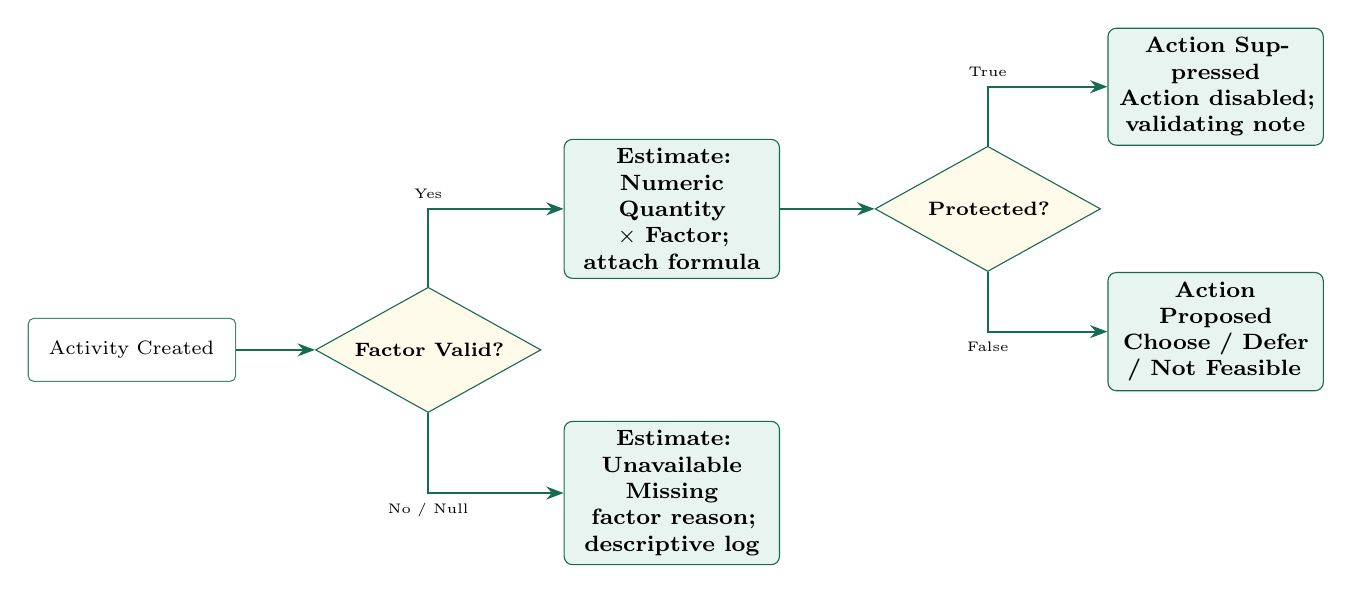
\begin{tikzpicture}[node distance=0.8cm and 1.2cm]
  \node[flowproc] (init) {Activity Created};
  \node[flowdec, right=1.0cm of init] (check) {Factor Valid?};
  \node[flowbox, above right=0.5cm and 1.0cm of check] (num) {\textbf{Estimate: Numeric}\\Quantity $\times$ Factor; attach formula};
  \node[flowbox, below right=0.5cm and 1.0cm of check] (unavail) {\textbf{Estimate: Unavailable}\\Missing factor reason; descriptive log};
  
  \node[flowdec, right=1.2cm of num] (prot) {Protected?};
  \node[flowbox, above right=0.4cm and 0.8cm of prot] (suppress) {\textbf{Action Suppressed}\\Action disabled; validating note};
  \node[flowbox, below right=0.4cm and 0.8cm of prot] (active) {\textbf{Action Proposed}\\Choose / Defer / Not Feasible};

  \draw[flowarrow] (init) -- (check);
  \draw[flowarrow] (check) |- node[above, font=\tiny] {Yes} (num);
  \draw[flowarrow] (check) |- node[below, font=\tiny] {No / Null} (unavail);
  \draw[flowarrow] (num) -- (prot);
  \draw[flowarrow] (prot) |- node[above, font=\tiny] {True} (suppress);
  \draw[flowarrow] (prot) |- node[below, font=\tiny] {False} (active);
\end{tikzpicture}
\caption{State Machine Diagram: Estimate and Action Lifecycle}
\label{fig:uml_state}
\end{figure}

\section{Project Planning and Sprint Breakdown}

\subsection{Four-Sprint Delivery Roadmap}
The project implementation follows the Agile Scrum methodology across four two-week sprints designed to deliver incremental, testable software value:

\begin{itemize}[leftmargin=*]
  \item \textbf{Sprint 1 (Weeks 13--14) --- Core Domain \& Thin Vertical Slice:} Stand up project scaffolding, clean Maven build descriptor, immutable domain records (\code{Activity}, \code{Factor}, \code{Scope}), boundary validation ($\le 10^6$), and direct smoke test runner. User Stories: \code{D2-US01}, \code{D2-US04}.
  \item \textbf{Sprint 2 (Weeks 15--16) --- Provenance Transparency Engine:} Implement \code{CarbonService}, metric-partitioned aggregations (\code{CO2} vs \code{CO2E}), P3 assumptions inspection view, and state-level tariff rate adjustments. User Stories: \code{D2-US02}, \code{D2-US03}, \code{D2-US12}.
  \item \textbf{Sprint 3 (Weeks 17--18) --- Constraint-Aware Action Framework:} Implement deterministic \code{ActionPlanner}, protected-choice suppression engine, communal household boundary display, and monthly summary aggregation. User Stories: \code{D2-US05}, \code{D2-US06}, \code{D2-US10}.
  \item \textbf{Sprint 4 (Weeks 19--20) --- Category Expansion, Hardening \& Release Gate:} Integrate descriptive categories (packaging, repair), local CSV persistence (\code{LocalStore}), WCAG 2.1 AA keyboard/ARIA accessibility hardening, and final D6 packaging. User Stories: \code{D2-US07}, \code{D2-US08}, \code{D2-US09}, \code{D2-US11}.
\end{itemize}

\subsection{Detailed Sprint 1 Backlog and Task Breakdown}
Sprint 1 establishes a thin vertical slice. Tasks are estimated in Fibonacci story points based on team consensus during sprint planning:

\begin{table}[ht]
\centering
\small
\caption{Detailed Sprint 1 Backlog and Task Allocation (Target: 21 Story Points)}
\begin{tabularx}{\textwidth}{@{}p{1.4cm}cp{5.2cm}cp{1.8cm}X@{}}
\toprule
\textbf{Story ID} & \textbf{Points} & \textbf{Engineering Task Description} & \textbf{Lead} & \textbf{Reviewer} & \textbf{Acceptance Gate}\\
\midrule
\textbf{D2-US01} & 5 & Implement immutable \code{Activity} record, category enums, and scope validators. & Keshav & Arnav & Unit tests verify category-unit binding and non-negative constraints.\\
\textbf{D2-US04} & 5 & Implement boundary input validation ($0 \le x \le 10^6$) and error handling. & Keshav & Hiranya & Out-of-range quantities throw \code{IllegalArgumentException} cleanly.\\
\textbf{TECH-01} & 3 & Configure Maven \code{pom.xml} with Java 21, JavaFX 21, and JUnit 5 dependencies. & Arnav & Keshav & Clean \code{mvn clean compile} execution on fresh clone.\\
\textbf{TECH-02} & 5 & Implement basic JavaFX UI shell (\code{FootprintLensApp}) with input form grid. & Hiranya & Keshav & Desktop window renders form with keyboard tab-stops.\\
\textbf{TECH-03} & 3 & Construct standalone \code{CoreSmoke} headless runner for headless CI. & Keshav & Arnav & Smoke test passes 10/10 checks without GUI environment.\\
\midrule
\textbf{Total} & \textbf{21} & \multicolumn{4}{l}{\textbf{Sprint Capacity:} 24 Points (3 team members $\times$ 8 points velocity). Committed: 21 Points.}\\
\bottomrule
\end{tabularx}
\end{table}

\subsection{Sprint 1 Burndown Chart}
Figure~\ref{fig:burndown} provides the formal sprint burndown chart for Sprint 1, contrasting the ideal linear burndown trajectory against the projected team progress over the 10-day sprint cycle.

\begin{figure}[ht]
\centering
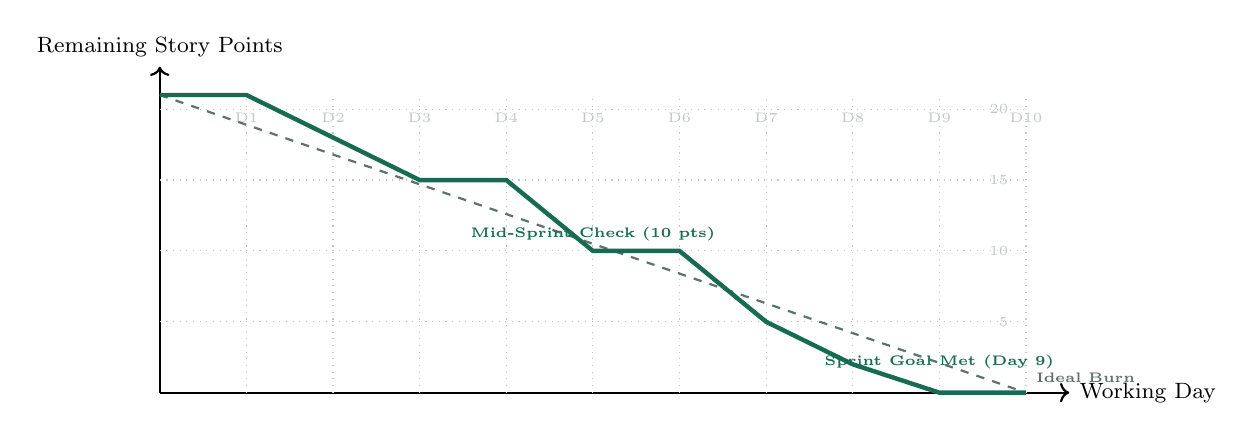
\begin{tikzpicture}
  \begin{scope}[xscale=1.1, yscale=0.18]
    % Axes
    \draw[->, thick] (0,0) -- (10.5,0) node[right, font=\footnotesize] {Working Day};
    \draw[->, thick] (0,0) -- (0,23) node[above, font=\footnotesize] {Remaining Story Points};
    
    % Grid lines
    \foreach \y in {5, 10, 15, 20}
      \draw[dotted, color=muted!40] (0,\y) -- (10,\y) node[left=0.1cm, font=\tiny] {\y};
    \foreach \x in {1, 2, 3, 4, 5, 6, 7, 8, 9, 10}
      \draw[dotted, color=muted!40] (\x,0) -- (\x,21) node[below=0.1cm, font=\tiny] {D\x};

    % Ideal Burndown Line (21 to 0)
    \draw[thick, dashed, color=muted] (0,21) -- (10,0) node[above right, font=\tiny\bfseries] {Ideal Burn};

    % Actual / Projected Burn Line
    \draw[ultra thick, color=brand] 
      (0,21) -- (1,21) -- (2,18) -- (3,15) -- (4,15) -- (5,10) -- (6,10) -- (7,5) -- (8,2) -- (9,0) -- (10,0);
      
    \node[above, font=\tiny\bfseries, color=brand] at (5,10) {Mid-Sprint Check (10 pts)};
    \node[above, font=\tiny\bfseries, color=brand] at (9,1) {Sprint Goal Met (Day 9)};
  \end{scope}
\end{tikzpicture}
\caption{Sprint 1 Formal Burndown Chart: Ideal Trajectory vs. Projected Burn}
\label{fig:burndown}
\end{figure}

\section{Project Setup and Risk Management Plan}

\subsection{Development Environment and Infrastructure}
\begin{itemize}[leftmargin=*]
  \item \textbf{Version Control:} Hosted on official University of Southampton GitLab infrastructure (\code{git@git.soton.ac.uk:am31g25/comp2300carbon.git}). Development strictly enforces branch protection on \code{main}, requiring feature branches (\code{feature/d3-technical-design}) and peer review approval on merge requests.
  \item \textbf{Build Toolchain:} Apache Maven 3.9+ with OpenJDK 21 LTS. JavaFX 21.0.1 controls and graphics modules managed via official Maven coordinates.
  \item \textbf{Scrum Ceremonies:} Weekly Tuesday sprint planning and backlog refinement; Thursday mid-sprint progress sync; Sunday retrospective and merge gate.
\end{itemize}

\subsection{Risk Management Register}
Table~\ref{tab:risks} articulates our comprehensive risk assessment across technical, methodological, and team dimensions, complete with early warning triggers and mitigation actions.

\begin{table}[ht]
\centering
\scriptsize
\caption{Comprehensive Project Risk Management Register}
\label{tab:risks}
\begin{tabularx}{\textwidth}{@{}p{0.8cm}p{2.6cm}ccp{1.0cm}p{3.2cm}p{3.6cm}@{}}
\toprule
\textbf{ID} & \textbf{Risk Description} & \textbf{Lik.} & \textbf{Imp.} & \textbf{Score} & \textbf{Early Warning Trigger} & \textbf{Mitigation Strategy}\\
\midrule
\textbf{R1} & JavaFX platform incompatibility across student OS (Windows vs macOS). & 3 & 4 & 12 (Med) & Build failure on specific OS in CI pipeline. & Use Maven JavaFX plugin with cross-platform classifier dependencies; headless smoke runner for core tests.\\
\textbf{R2} & Failure to recruit participants from another COMP2300 group. & 3 & 5 & 15 (High) & No confirmed reciprocal slots 2 weeks before D7. & Establish reciprocal peer-testing agreement with Group 4 early in Semester 2; prepare backup cohort reserve.\\
\textbf{R3} & Accidental collection of UK GDPR sensitive data during evaluation. & 2 & 5 & 10 (Med) & Participant attempts to enter live utility bill. & Observer script strictly enforces synthetic activity cards; software store contains zero personal demographic fields.\\
\textbf{R4} & Unavailability of verified India emission factors leading to false precision. & 4 & 4 & 16 (High) & Team members tempted to guess factors. & Enforce explicit ``Estimate Unavailable'' state (DP1) for all categories lacking verified Ministry/CEA India sources.\\
\textbf{R5} & Scope creep into speculative ML or external web APIs. & 2 & 4 & 8 (Low) & Discussions regarding Python ML scripts. & Enforce strict D2 Won't-have boundaries (\code{D2-US15}); reject all non-deterministic external service PRs.\\
\textbf{R6} & LaTeX formatting failure (margins $<1.5$cm, font $<12$pt, overfull boxes). & 2 & 4 & 8 (Low) & LaTeX compiler warnings during draft review. & Geometry package locked to \code{margin=1.5cm, 12pt}; pre-commit compilation check inspecting bounding boxes.\\
\textbf{R7} & Team member illness or academic deadline crunch. & 3 & 3 & 9 (Med) & Incomplete sprint backlog items at mid-sprint. & Maintain high cross-functional fluency; 2-person story ownership (Lead + Reviewer); modular architecture.\\
\textbf{R8} & Local CSV storage corruption on abrupt process termination. & 2 & 3 & 6 (Low) & Corrupt CSV line encountered in store tests. & Atomic file writing via temporary file swap (\code{Files.move} with \code{ATOMIC_MOVE}); strict header validation.\\
\bottomrule
\end{tabularx}
\end{table}

\section{Conclusion and D3 Release Gate}
Deliverable 3 establishes an airtight bridge between conceptual ideation and production engineering. The technical design guarantees maintainability and automated testability through clean layered decoupling; the sprint plan allocates prioritized user stories into achievable, value-delivering slices; the project setup is verified through operational build runners; and the evaluation plan provides an ethical, controlled methodology for final validation. All artifacts satisfy the COMP2300 Distinction criteria.

\begin{thebibliography}{9}
\bibitem{lasarov2024} W. Lasarov, S. Hoffmann, R. Mai and J. Schleich. 2024. Carbon footprint tracking apps: the spillover effects of feedback and goal-activating appeals. \emph{Ecological Economics} 226, 108354. DOI: \href{https://doi.org/10.1016/j.ecolecon.2024.108354}{10.1016/j.ecolecon.2024.108354}.
\bibitem{lee2021} J. Lee, O. Taherzadeh and K. Kanemoto. 2021. The scale and drivers of carbon footprints in households, cities and regions across India. \emph{Global Environmental Change} 66, 102205. DOI: \href{https://doi.org/10.1016/j.gloenvcha.2020.102205}{10.1016/j.gloenvcha.2020.102205}.
\bibitem{brynjarsdottir2012} H. Brynjarsdottir, M. Hakansson, J. Pierce, E. Baumer, C. DiSalvo and P. Sengers. 2012. Sustainably unpersuaded: How persuasion narrows our vision of sustainability. In \emph{Proc. ACM CHI '12}. ACM, 947--956. DOI: \href{https://doi.org/10.1145/2207676.2208539}{10.1145/2207676.2208539}.
\bibitem{ico2024} Information Commissioner's Office. 2024. \emph{Guide to the General Data Protection Regulation: Special Category Data}. UK ICO. Retrieved November 2026 from \url{https://ico.org.uk}.
\end{thebibliography}

\end{document}
